\documentclass[a4paper,11pt]{article}
\usepackage[utf8]{inputenc}
\usepackage[T1]{fontenc}
\usepackage[french]{babel}
\usepackage{makeidx}
\usepackage{textcomp}
\usepackage{graphicx}
\usepackage{mathtools,amssymb,amsthm}
\usepackage{lmodern}
\usepackage{multirow}
\usepackage{array}
\usepackage{longtable}

\title{TER 2019 - Spécifications}
\author{Maxime Gonthier - Benjamin Guillot - Laureline Martin}
\begin{document}
	\pagenumbering{gobble}\clearpage
	\maketitle

\newpage
\tableofcontents

\newpage
\section{Introduction}
Dans la société actuelle les transports en communs prennent une part de plus en plus importante dans nos déplacements. Bien que pratique et plus écologique, ils sont toujours relativement pleins et donc peu agréable.\\
 L'objectif d'un bureau des temps est de réduire la congestion à l'intérieur de ces transports, c'est à dire de réduire le nombre de personnes présentent en même temps dans un transport. 
Notre objectif est donc de faire ce travail en partant d'un cas concret, celui de la ligne de bus R reliant la gare de Versailles-Chantier à l'université Versailles-Saint Quentin.\\
Pour ce faire, nous allons influer sur les emplois du temps de l'université en modifiant les heures de début de cours sur une journée afin de voir si la congestion est susceptible de baisser dans la ligne de bus après ces modifications.\\
A la fin du projet le but est de fournir une planification de l'emploi du temps de l'université sur une journée, c'est a dire les début de chaque cours.
\section{Modélisation des données en entrée}
	On va répartir les données concernant la fac en 4 modules.\\
	Un module est une classe et des fonctions nécessaire à la modélisation d'un acteur essentiel du projet. Par la suite les modules seront reliées entre eux et s'appelleront mutuellement.
	\begin{itemize}
		\item Module cours
		\item Module salle d'enseignement
		\item Module étudiant
		\item Module professeur
	\end{itemize}
	\subsection{Module Cours}
		Le module cours est une classe représentant un cours sur un temps donné.\\
		Lors des affectations, on modifiera pour chaque instance a deplacer l'horaire de début.\\
		\subsubsection{Classe Cours}
		\begin{enumerate}
			\item num\_cours :  un entier (identifiant unique)
			\item duree : un entier -représente la durée du cours en minutes-
			\item liste\_etu : un tableau d'entier qui contient les numero des étudiants participant à ce cours. On calcul le nombre d'étudiants participants au cours à partir de cette liste.
			\item type\_salle : un entier, 0 pour une salle de TP et 1 pour un autre salle (on pourra ajouter d'autres type de salle si necessaire).
			\item num\_salle : un entier (identifiant unique représentant la salle)
			\item num\_ens : un entier désignant le professeur donnant ce cours(identifiant unique représentant le professeur)
			\item debut : un entier. On divise le temps d'ouverture de l'université en créneau de 15 minutes, chaque entier représente le début d'un bloc de 15 minutes. 
			\item liste\_ens : une liste contenant les identifiants des professeurs pouvant enseigner ce cours.
		\end{enumerate}
	\subsection{Module Salle d'enseignement}
		Le module salle représente la localisation du cours sur un temps donné.
		\subsubsection{Classe Salle}
		\begin{enumerate}
			\item num\_salle : un entier (identifiant unique)
			\item localisation : un entier -0 pour proche de l'arrêt de bus desservant l'université, 1 pour modérément éloigné, 2 pour éloigné-. 
			\item type\_salle : un entier, 0 pour une salle de TP et 1 pour une autre salle (on pourra ajouter d'autres type de salle si necessaire).
			\item capacite : un entier désigant le nombre maximal d'étudiant que peut contenir la salle	
		\end{enumerate}
		\subsubsection{Matrice d'adjacence entre les salles}
	Cette matrice va indiquer la distance entre deux salles. Elle est symétrique. Si la distance prend moins de 15 min à parcourir a pied on met 0.
	Entre 15 et 30 min on met 1. Plus de 30 min on met 2.
		\subsubsection{Matrice d'adjacence entre salles et arrêt de bus}
		De même mais cette fois la matrice a une seule colonne représentant l'arrêt de bus desservant l'université.
		On regarde alors le temps que l'ont met pour aller de l'arrêt de bus a la salle et on remplit de la même manière que pour la matrice précédente.
	\subsection{Module Etudiant}
		Le module étudiant représente un étudiant.
		\subsubsection{Classe Étudiants}
		\begin{enumerate}
			\item num\_etu : un entier (identifiant unique)
			\item distance : un entier qui représente la distance entre le domicile de l'étuidant et l'université, 0 si l'étudiant habite a moins de 15 min de la fac, 1 si il habite entre 15 et 45 min de la fac, 2 sinon.
			\item contrainte : un entier qui représente la contrainte faible à laquelle un étudiant peu être associée. 0 s'il n'est associé à aucune contrainte, 1 s'il associé à la contrainte travail, 2 s'il est associé à la contrainte enfant, 3 s'il est associé aux deux contraintes précédentes. 
			\item heure\_debut : un entier, représente l'heure du premier cours de la journée de l'étudiant.
			\end{enumerate}
	\subsection{Module Professeur}
		Le module professeur représente un professeur.
		\subsubsection{Classe Professeur}
		\begin{enumerate}
			\item num\_ens : un entier (identifiant unique)
			\item plage : un tableau dont chaque case représente un bloc horaire (15 min par exemple)
			Si xi vaut 0 alors c'est l'horaire du début de la disponibilité, si xi vaut 1 c'est la fin de la disponibilité du professeur.
			\end{enumerate}
	\subsection{Liens entre les modules}
		\centerline{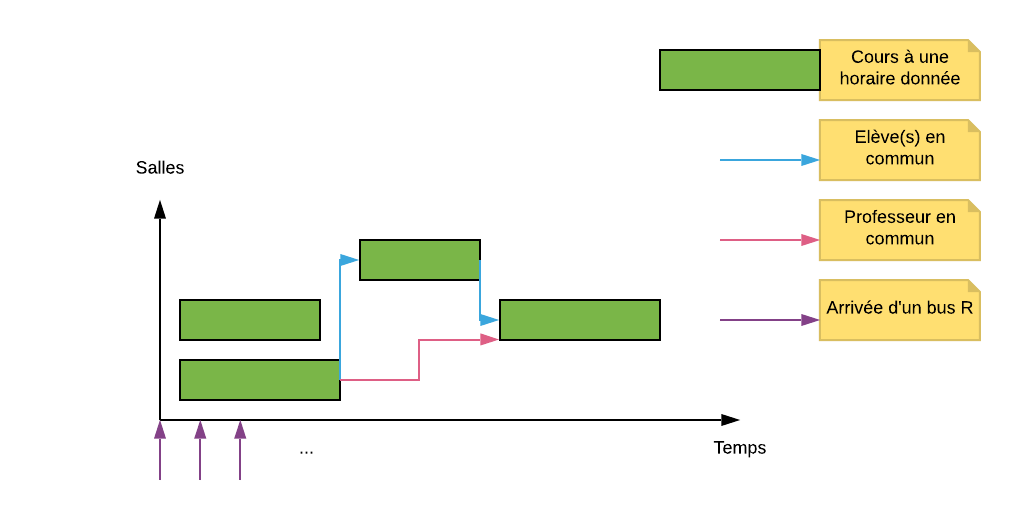
\includegraphics[scale=0.5]{modelter.png}}
		Modélisation.\\

\section{Module Contraintes}
	Pour optimiser, nous faisons face à plusieurs contraintes, toutes ne sont pas 
	de même "importances". Nous allons donc devoir définir un ordre de priorité sur 
	les contraintes, ainsi lors de l'optimisation par notre algorithme, nous 
	pourrons ajuster et obtenir de meilleurs résultats même si certaines contraintes
	"faibles" sont violées.\\
	\subsection{Contraintes dures}
			\subsubsection{Entre deux cours}
				\begin{enumerate}
					\item Si deux cours utilisent la même salle à des horaires qui se chevauchent ou
					\item Si il y a des élèves en commun sur deux cours dont les horaires se chevauchent.
					\item Si le temps laissé entre les deux cours est inférieur au temps nécessaire pour relier les deux salle de classe (à pied).
				\end{enumerate}
			\subsubsection{Entre un cours et un professeur}
				\begin{enumerate}
					\item Le professeur doit pouvoir enseigner ce cours. D'où la création de la liste de professeur pouvant enseigner un cours dans le module cours.
					\item 	On regarde aussi si la plage de disponibilité du professeur correspond à l'horaire du cours.
				\end{enumerate}
			\subsubsection{Entre un cours et une salle}
				\begin{enumerate}
					\item 	La salle doit avoir une capacité supérieure ou égale au nombre d'élèves suivant le cours et doit correspondre au type de salle dont le cours a besoin.
				\end{enumerate}
	On ne précise pas la contraintes entre cours et étudiant car un étudiant est défini par ses cours.
	\subsection{Contraintes faibles}
		\begin{enumerate}
			\item Avoir une personne à charge ce qui impose un horaire le matin et/ou le soir.
			Exemple : Sois X l'heure de début d'un cours, si un enfant doit être déposé à l'école à 9h on a : X > 9 + (indice de distance de cet étudiant)*30 min
			Sois Y l'heure de fin d'un cours, si un enfant doit être récupéré à l'école à 17h on a : Y < 17 - (indice de distance de cet étudiant)*30 min
			\item Avoir un travail, cela impose la même chose que la contraintes précédentes
		\end{enumerate}
\section{Affectation}
	On va affecter chaque cours à un horaires sans prendre en compte les transports. On ne va utiliser que les contraintes énoncés précédemment. \\
	A chaque cours on affec		te une horaire de début (l'horaire de fin est calculé en conséquence), tel que les contraintes dures sont validées.
	On va utiliser une heuristique tabou. On commence avec un emploi du temps par défaut. Le voisinage correspond à la modification d'un cours. A chaque itération on recalcule le nombre de contraintes violées. Un optimum local sera une solution viable, c'est à dire qui ne viole pas les contraintes dures.
	(Si les solutions trouvées boucle (c'est à dire si les résultats restent similaires) alors on va éloigner le voisnage A REDIRE MIEUX)
	(Relier l'affectation aux bus)	
\section{Implémentation des bus}
	Pour les transports, on supposera que chaque élève arrivera par le bus précédant le début du premier cours de sa journée. 
	De cette manière a chaque itération de l'affectation des cours, on pourra recalculer la congestion de chaque bus
	(qui sera utilisé comme fonction objectif du projet une fois les transport implémentés).La congestion sera représenté par le maximun du dépassement de la limite de confort du bus lors du trajet.
	On utilisera la fonction $$calcul congestion$$ décrite ci dessous pour calculer cette valeur pour chaque bus.
	
\section{Les fonctions principales}
	\subsection{Flexibilité}
		\subsubsection{Calcul flexibilité étudiant}
		Cette fonction prend en entrée la distance entre le domicile de l'étudiant et l'université ainsi que les contraintes
		associées à l'étudiant (si il en possède). La fonction calcule et renvoie la flexibilité de l'étudiant.
		$$flexibilité\_etu  = distance + 2*(contrainte)$$
		\subsubsection{Calcul indice de flexibilité}
		Cette fonction prendra en entrée la flexibilité de chaque étudiant assistant à un cours donné et en fera la somme. 
		Un indice de flexibilité est ainsi calculé, cette modelisation a pour but de favoriser les cours ayant le plus d'etudiants.\\
		$$flexibilité\_cours = \Sigma_{i = 0}^{nb\_etu} flexibilité\_etu$$
	\subsection{Verifications des contraintes}
		\subsubsection{entre Professeur et Cours}
			Prend en entrée un Professeur et un Cours.\\
			On vérifie que $num\_ens$ appartient à la liste $liste\_ens$ qui contient les identifiant des professeurs pouvant enseigner ce cours.\\
			Vérifie également que la plage de disponibilité $plage$ est compatible avec l'horaire de début $debut$ + la durée $durée$ du cours .
		\subsubsection{entre Cours et Cours}
			Prend en entrée deux Cours.\\
			On vérifie qu'il n'y a pas d'intersection entre :\\
			\begin{itemize}
				\item Les listes $liste\_etu$ de chaque cours si les horaires se chevauchent.
				\item Les numéro de salle $num\_salle$ si les horaires se chevauchent.
				\item On vérifie à l'aide de la matrice d'adjacence des salles que le temps entre deux cours ayant des étudiants en commun est supérieur au temps nécessaire pour rallier les deux salles.
			\end{itemize}
		\subsubsection{entre Cours et Salle}
			Prend en entrée un Cours et une Salle.
			On vérifie que le nombre d'étudiants (calculé à partir de $liste\_etu$) ne dépasse pas la capacité $capacite$ de la Salle.
			On vérifie que le type $type\_salle$ du Cours correspond bien au type $type\_salle$ de la Salle utilisée.
		\subsubsection{Verification des contraintes faibles}
			Prend en entrée un Cours et un Étudiant.
			On vérifie que l'heure de début du premier cours ou du dernier (+ sa durée) de l'étudiant laisse une assez grande marge en fonction de sa contrainte faible.
			Si possible cette valeur sera prise en compte pour modifier les emploi du temps et faire commencer (au plus tard) les cours à 9h, et finir (au plus tôt) à 17h.
		\subsection{Fonctions répétés à chaque itération de l'algorithme}
			\subsubsection{Calcul congestion}
				Prend en entrée les élèves, un par un.
				Pour chaque élève on regarde l'heure du début de son premier cours ainsi que la distance entre la salle de ce cours et l'arrêt de bus. 
				Ainsi on en déduit le bus que cet étudiant doit emprunter. On fais ensuite la somme des maximums du dépassement de la limite
				de confort pour chaque bus. Cette valeur sera la variable $$congeston$$.
			\subsubsection{Nouvelle planification}
				On prend en entrée Cours.
				On modifie l'heure de début de un ou plusieurs cours. Pour faire cela on va s'inspirer d'une heuristique tabou.
				On va donc à partir de la planification initiale explorer son voisnage c'est à dire des explorer planifications identiques à l'exception
				de un ou deux horaires de début de cours.
				Les positions explorées seront stockées dans un fichier de sortie répertoriant les horaires de début de chaque cours.
				Le numéro des cours ayant été modifié sera également stocké.
			\subsubsection{Nouveau bus}
				On prend en entrée les cours qui ont été modifié.
				On va alors affecter a chaque élève dont l'heure du premier cours a été modifié le bus y correspondant.

\section{Fonctionemment global de l'application}
	\subsection{Données initiales}
		On considère que les données fournit en entrées sont : 
		\begin{itemize}
				\item Une planification de base de la journée, c'est à dire un horaire de déut pour chaque cours.
				\item Les cours, les élèves, les professeurs et les salles d'enseignements
				\item Le nombre de bus total sur la journée ainsi que leurs horaires d'arrivée à l'université
				\item Les distances entre les salles et les distances entre les salles et l'arrêt de bus de l'université.
			\end{itemize}
	\subsection{Itérations}
		A chaque itérations on va :
		\begin{itemize}
				\item Créer une nouvelle planification en appellant la fonction $$Nouvelle planification$$.
				\item En déduire les bus dont les voyageurs ont été modifié avec la fonction $$Nouveau bus$$.
				\item Calculer la congestion avec la fonction $$Calcul congestion$$.
				\item Evaluation et stockage de la planification et de sa congestion associé dans un fichier de sortie.
			\end{itemize}
	\subsection{Arrêt de l'application}
		L'application s'arrêtera sois à partir d'un certains nombre d'itérations données, sois si la congestion
		converge.		
\section{Métrique d'évaluation}
	Chaque planification sera évalué selon deux critères. Dans un premier temps on va répertorier le nombre de contraintes faibles violées.
	Dans un second temps on va regarder le résultat de la fonction $$calcul congestion$$.
	Un score sera calculé ainsi : 
	$$score  = congestion + nb\_contrfaible$$

\end{document}
